\section{Tree caching with dependencies}
The problem we consider (called \textit{tree caching problem})is an extension 
of classic caching problem with bypassing that was recalled in section 2. The 
main difference is that requested items have inter-dependencies. Specifically, 
universe forms rooted tree $T$ and the items requested are placed in its nodes 
and whenever $v \in T$ is fetched all of its descendants $T(v)$ that are not in 
cache have to be fetched at the same time. We say that the cache with property 
described above is \textit{bottom-contiguous}.

Moreover, we consider two types of requests: \textit{negative} and 
\textit{positive}. If incoming request is positive we pay 1 if it is 
not present in the cache (so the same as in most considered settings). On the 
other hand we pay for negative requests if the item is cached (so in opposite 
situation). After serving of any request we can reorganize cache paying 
$\alpha \geq 1$ for every element evicted or fetched. 

The goal is to minimize the cost obtained by online algorithm solving this 
problem. We present a deterministic algorithm \textbf{TRC} which we prove is 
$O(h(T) \times R)$-competitive where $h(T)$ is height of input tree and $R = 
k_{ONL}/(k_{ONL} - k_{OPT} +1$ with $k_{ONL}$ and $k_{OPT}$ being size of 
online and optimal offline algorithm cache.

\subsection{Model}
\begin{wrapfigure}{r}{0.6\textwidth}
\begin{postscript}

\psscalebox{0.6 0.6} % Change this value to rescale the drawing.
{
\begin{pspicture}(0,-4.0099998)(12.562361,4.0099998)
\definecolor{colour0}{rgb}{0.78431374,0.78431374,0.78431374}
\psbezier[linecolor=black, linewidth=0.04, 
fillstyle=solid,fillcolor=colour0](4.8323607,3.9899998)(3.8323605,
3.9899998)(0.046042196,0.2078214)(0.8323605,-0.41000015)(1.6186789,
-1.0278217)(9.759687,-1.1499403)(10.432361,-0.41000015)(11.105033,
0.32993993)(5.8323607,3.9899998)(4.8323607,3.9899998)
\pscircle[linecolor=black, linewidth=0.04, fillstyle=solid,fillcolor=black, 
dimen=outer](4.8323607,2.79){0.4}
\pscircle[linecolor=black, linewidth=0.04, fillstyle=solid,fillcolor=black, 
dimen=outer](3.2323606,1.9899999){0.4}
\pscircle[linecolor=black, linewidth=0.04, fillstyle=solid,fillcolor=black, 
dimen=outer](4.8323607,1.1899998){0.4}
\pscircle[linecolor=black, linewidth=0.04, fillstyle=solid,fillcolor=black, 
dimen=outer](6.4323606,1.9899999){0.4}
\pscircle[linecolor=black, linewidth=0.04, fillstyle=solid,fillcolor=black, 
dimen=outer](8.03236,1.1899998){0.4}
\pscircle[linecolor=black, linewidth=0.04, fillstyle=solid,fillcolor=black, 
dimen=outer](7.6323605,-0.41000015){0.4}
\pscircle[linecolor=black, linewidth=0.04, fillstyle=solid,fillcolor=black, 
dimen=outer](9.232361,-0.0100001525){0.4}
\psline[linecolor=black, linewidth=0.04](4.8323607,2.79)(3.2323606,1.9899999)
\psline[linecolor=black, linewidth=0.04](4.8323607,2.79)(4.8323607,1.1899998)
\psline[linecolor=black, 
linewidth=0.04](4.8323607,2.79)(6.4323606,1.9899999)(6.4323606,1.9899999)
\psline[linecolor=black, 
linewidth=0.04](6.4323606,1.9899999)(8.03236,1.1899998)(7.6323605,
-0.41000015)(8.03236,1.1899998)(9.232361,-0.0100001525)(9.232361,-0.41000015)
\psline[linecolor=black, 
linewidth=0.04](3.2323606,1.9899999)(3.2323606,1.9899999)
\psline[linecolor=black, 
linewidth=0.04](4.8323607,2.79)(4.8323607,2.79)(4.8323607,2.79)
\pstriangle[linecolor=black, linewidth=0.06, 
dimen=outer](1.2323605,-3.6100001)(2.4,2.8)
\pstriangle[linecolor=black, linewidth=0.06, 
dimen=outer](4.8323607,-3.6100001)(2.4,2.8)
\psline[linecolor=black, 
linewidth=0.04](4.8323607,0.78999984)(4.8323607,-0.8100002)(4.8323607,
-0.8100002)
\pstriangle[linecolor=black, linewidth=0.06, 
dimen=outer](9.232361,-3.6100001)(2.4,2.8)
\psline[linecolor=black, 
linewidth=0.04](2.8323605,-0.0100001525)(2.8323605,-0.0100001525)(2.8323605,
-0.0100001525)(2.8323605,-0.0100001525)
\rput(11.63236,1.9899999){Tree cap}
\rput(9.232361,-0.0100001525){\textcolor{white}{\textbf{r}}}
\pspolygon[linecolor=black, linewidth=0.04, fillstyle=vlines, 
hatchwidth=0.028222222, hatchangle=0.0, 
hatchsep=0.1411111](2.4323606,-3.6100001)(1.6323606,-2.41)(1.2323605,
-2.8100002)(0.8323605,-2.0100002)(0.032360535,-3.6100001)(0.032360535,
-3.6100001)
\pspolygon[linecolor=black, linewidth=0.04, fillstyle=vlines, 
hatchwidth=0.028222222, hatchangle=0.0, 
hatchsep=0.1411111](4.4323606,-3.6100001)(4.8323607,-2.41)(6.0323606,
-3.6100001)(6.0323606,-3.6100001)
\psframe[linecolor=black, linewidth=0.04, fillstyle=vlines, 
hatchwidth=0.028222222, hatchangle=0.0, hatchsep=0.1411111, 
dimen=outer](10.432361,3.1899998)(9.63236,2.3899999)
\rput(11.63236,2.79){Valid cache }
\psline[linecolor=black, 
linewidth=0.04](9.232361,-1.6100001)(9.232361,-1.6100001)(9.232361,
-1.6100001)(9.232361,-1.6100001)
\psline[linecolor=black, 
linewidth=0.04](9.232361,-0.0100001525)(9.232361,-0.8100002)(9.232361,
-0.8100002)
\pstriangle[linecolor=black, linewidth=0.06, linestyle=dotted, 
dotsep=0.10583334cm, fillstyle=vlines, hatchwidth=0.02, hatchangle=0.0, 
hatchsep=0.2212, dimen=outer](9.232361,-4.01)(4.0,5.2)
\psline[linecolor=black, 
linewidth=0.04](3.2323606,1.9899999)(1.2323605,-0.8100002)(1.2323605,-0.8100002)
\psline[linecolor=black, 
linewidth=0.04](3.2323606,1.1899998)(3.2323606,1.1899998)
\psline[linecolor=black, 
linewidth=0.04](4.8323607,3.59)(4.8323607,3.59)(4.8323607,3.59)(4.8323607,3.59)
\psframe[linecolor=black, linewidth=0.04, fillstyle=solid,fillcolor=colour0, 
dimen=outer](10.432361,2.3899999)(9.63236,1.5899998)
\psframe[linecolor=black, linewidth=0.064, linestyle=dotted, 
dotsep=0.10583334cm, fillstyle=solid, 
dimen=outer](10.432361,3.9899998)(9.63236,3.1899998)
\rput(11.63236,3.59){T(r)}
\end{pspicture}
}

\end{postscript}
\caption{Visualization of definitions.}
\label{fig:TreeCacheDefinitions}
\end{wrapfigure}
For ease of future algorithm description and readability of proofs we introduce 
some useful definitions. First of all by $T(r)$ we mean subtree of $T$ rooted 
in $r$ and by $h(T)$ height of tree. \textit{Tree cap} is a tree $T_c \subseteq 
T$ such that root $r$ of $T$ belongs to it and $v \in T_c$ implies that all the 
nodes on the path from $v$ to $r$ belong to $T_c$. We say that set $C \subseteq 
T$ is \textit{bottom contiguous} if $v \in C$ implies $T(v) \subseteq C$ and we 
say that set $C$ \textit{valid cache state}. Notice that it is not dependent on 
cache size so $C$ ca be valid cache state and not fit into cache size the same 
time.

The \textbf{TRC} algorithm, after each request, can change the state of cache, 
but the only possible changes have to leave the cache in valid state. 
Depending on the character of change (eviction vs. fetch) we can apply for cache 
$C$ either \textit{valid negative changeset} or \textit{valid positive 
changeset}. The valid positive changeset $X$ (think of it as a set that can be 
fetched) is a set for which $X \cap C = \varnothing$ and $C \cup X$ 
is a valid cache state, the negative one (related to eviction) is a set $X 
\subseteq C$ such that $C \ X$ is valid cache state.

We process the input one by one and assume each request $\sigma(t)$ comes in 
time interval $(t-1, t)$, so the next request comes in time interval $(t, t + 
1)$ and so on. At time $t$ algorithm changes cache state from $C_{t}$ to 
$C_{t+1}$. Cache state is well defined for round $t$ (which contains time 
interval $(t-1, t)$), because as we see the cache may change only between 
rounds.

Some of the definition which appeared in this section are presented on figure 
~\ref{fig:TreeCacheDefinitions}.

\subsection{Algorithm TRC}

Before finally defining the \textbf{TRC} algorithm we bind to each node $v \in 
T$ a $bank_{t}(v)$ value. At the beginning of algorithm for each $v \in T$ we 
have $bank_{0}(v) = 0$. If node $v$ gets negative or positive request at 
time $t$ for which we pay 1 we increase $bank_{t}(v) = bank_{t-1}(v) + 1$, 
leaving the value for any other node unchanged (so for $v' \neq v 
bank_{t-1}(v') = bank_{t}(v')$). When we change the state of node $v$ (either 
evict or fetch it into cache) we clear its bank value. For set of nodes $V 
\subseteq T$, we denote sum $\sum_{v \in V} bank_{t}(v)$ as $bank_{t}(V)$.

The \textbf{TRC} proceeds in phases. First phase starts at time 0 and at the 
start of each phase the \textbf{TRC} cache is empty. 
\begin{algorithm}
\caption{\textbf{TRC}}
\label{alg:TRC}
\begin{algorithmic}[1]
\ForAll{$t \in \{1 \ldots |\sigma|\}$}
  \State Serve request $\sigma(t)$.
  \State Compute $bank_t(v)$ values for $v \in T$.
  \If{exists valid changeset $X$ such that: \begin{itemize}
    \item $bank_t(X) \geq |X| \times \alpha$ (saturation),
    \item $bank_t(Y) < |Y| \times \alpha$ for any valid changeset $Y 
\varsupsetneq X$ (maximality):
\end{itemize}}
 \State Apply $X$.
 \If {cache size $k_{ONL}$ is exceeded}:
  \State Empty cache.
  \State Reset $bank_t$ values to be 0.
  \State Start new phase.
 \EndIf
 \EndIf
\EndFor
  \end{algorithmic}
\end{algorithm}

In line 6 of the algorithm above we do not actually exceed the cache. Instead 
we do not apply last valid changeset, empty the cache and start new phase. 
Every phase ends then whenever applying valid changeset $X$ would lead to cache 
being overloaded except of the last phase: this one can be \textit{unfinished}. 
If $P$ is a phase, by $begin_P$ and $end_P$ we denote time when the phase $P$ 
started and finished respectively.

\subsection{Analysis}
Throughout all the analysis we fix the input sequence $I$ and its division into 
phases. We compare \textbf{TRC} with \textbf{OPT} by analyzing both on a single 
phase $P$. By $k_P$ we denote the number of elements in \textbf{TRC's} cache 
after artificial fetch at $end_P$ but before all cache elements eviction.

We start with some basic properties of changesets. Then we introduce 
\textit{fields} which will help us proving algorithm's competitiveness.

\subsubsection{Elementary properties}
Remind that $C_t$ denotes the cache state of \textbf{TRC} at round $t$ and that 
any cache change takes place between rounds in discrete times. 
Having that in mind we prove that at any time there cannot be both saturated 
positive and negative changesets.
\begin{lemma}
\label{thm:lemma1}
 Fix phase $P$. For any $t \in \{begin_P +1, begin_P + 2, \ldots, end_P\}$. 
For any valid changeset $X$ for cache $C_t$ we have $bank_t(X) \leq |X| \cdot 
\alpha$ (1). Moreover changesets $Y$ for $C_t$ for which equality holds are 
all either positive or negative (2).
\end{lemma}
\begin{proof}
We prove this lemma by induction on $t$, starting with $t_1 = begin_P +1$. In 
that time there was only one request so for all $X$ being valid changeset 
$bank_{t_1} \leq 1$, which proves (1). For (2) see that the request can be both 
negative and positive.

To process with the induction step, first we prove following property:
\begin{property}
For any changeset $X$ for $C_{t+1}$ we have $bank_t(X) < |X| \cdot \alpha$.
\end{property}
We prove it only for $X$ being positive changeset. For negative ones the proof 
is symmetric. We consider three cases depending on the action taken by 
algorithm \textbf{TRC} at time $t$.
\begin{enumerate}
 \item \textbf{TRC} does not perform any action. That means that there was no 
saturated (saturation is defined in algorithm \ref{alg:TRC} above) changeset 
$X'$ for $C_t$ and $bank_t(X') \cdot \alpha$ for any $X'$. See that $C_t = 
C_{t+1}$, therefore property follows trivially in that case.
  \item \textbf{TRC} fetches $X'$, so $C_{t+1} = C_t \cup X'$. Assume the 
opposite, that there exists changeset $X$ for $C_{t+1}$ such that $bank_t(X) 
\geq |X| \cdot \alpha$. It implies that $X \cup X'$ is positive changeset for 
$C_t$ that might have been fetched instead of $X'$ at time $t$. That 
contradicts the maximality property of algorithm.
  \item \textbf{TRC} evicts $X'$, so $C_{t+1}  = C_t \setminus X'$. Assume 
again the opposite of the property. It gives, that $X'' = X \ X'$ is valid 
positive changeset for $C_t$ which is saturated, because $bank_t(X'') = 
bank_t(X) \geq |X| \cdot \alpha \geq |X''| \cdot \alpha$. We have both positive 
and negative saturated changeset for $C_t$ which contradicts induction 
assumption (2).
\end{enumerate}
This property implies the lemma for $t+1$ since we have strict inequalities for 
$C_{t+1}$. When request comes in round $t+1$ it is either positive or negative, 
so if it make a changset saturated it can be either positive or negative one. 
Only one request cames during the round, so strict inequalities can only change 
for equalities, so we have first part of lemma, too.
\end{proof}
The above lemma convince us that the algorithm is deterministic when choosing 
changeset to apply.

\subsubsection{Concept of fields}
First notice that whenever there is a positive (negative) request to element 
present (absent)in \textbf(TRC's) cache it neither influence the algorithm 
behaviour nor cost. Therefor from now on we assume that in phase $P$ there are 
no such requests.
We extend the space of requests from nodes to pairs of nodes and time $(v, t)$ 
calling them \textit{slots} and obtained space: \textit{event space}. If there 
is a request to node $v$ at time $t$ we say that slot $(v, t)$ is 
\textit{occupied}. We can then see each phase $P$ as set of occupied slots. 
Figure \ref{fig:spacial_temporal} might help to familiarize with above 
definitions.
\begin{figure}
 \begin{center}
  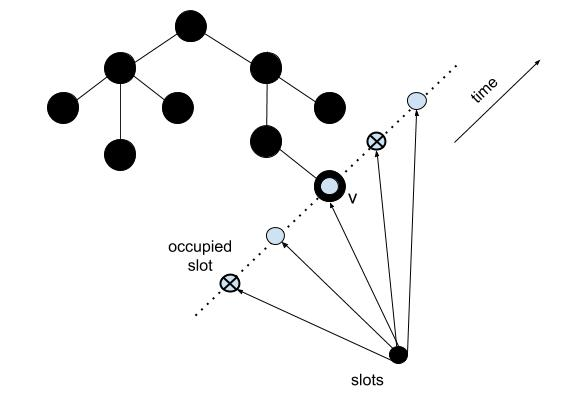
\includegraphics[width=0.7\textwidth]{spacial_temporal.jpg}
 \end{center}
 \caption{Event space for node $v$.}
 \label{fig:spacial_temporal}
\end{figure}

As we now know what event space and slots are, we can define $fields$. Fields 
form disjoint partition of phase $P$ (meaning partition of corresponding 
slots). Formally if $X_t$ is changeset applied by \textbf{TRC} at time $t$ we 
define related filed as:
$$ F^t = \{(v, t'): v \in X^t \wedge last_v^t < t' \leq t\},$$
where $last_v^{t'}$ denotes the last time strictly before $t'$ in phase $P$ 
when node $v$ changed its state in cache either by being fetched or evicted. If 
there was no such change for $v$ in phase $P$ we assign $last_v^{t'} = begin_P$.
$F^t$ is \textit{positive} if changeset $X_t$ is positive, symmetrically for 
\textit{negative}. We define $req(F^t)$ to be occupied slots from $F^t$. Notice 
that $req(F^t)$ all exactly the requests that 'payed' for changeset $X_t$. 
Together with Lemma \ref{thm:lemma1} we can summarize it in simple observation.
\begin{observe}
For field $F^t$ we have $req(F^t) = |X_t| \cdot \alpha$ and the requests 
in one field are either all positive or all negative.
\end{observe}
The rest of event space, occupied slots that does not belog to any field $F^t$ 
in phase $P$, we call \textit{open field} $F^{\inf}$. All fields except of an 
open field are denoted by $\mathcal{F}$ and $|\mathcal{F}| = \sum_{F^t \in 
\mathcal{F}} |X^t| \cdot \alpha$.
Additionaly for any field $F$, if $A$ is a set of nodes, $F \cap A = \{(v,t) 
\in F: v \in A$ and if $T$ is set of rounds $F \cap T = \{(v, t) \in F: t \in 
T\}$. To shorten notation we introduce $\tau$\textit{-restricted} subfields of 
$F^t$ as:
$$F^t_{\leq \tau} = F^t \cap {t': t' \leq \tau}.$$
We can think of it as sotopping time at $\tau$ and looking what slots are 
occupated up to this time in $F^t$.
Fields are hard to visualize in general case, so we present them on a 
Figure \ref{fig:fields} only for the case when the processed tree structure 
forms a line.
\begin{figure}
\label{fig:fields}
\begin{center}
  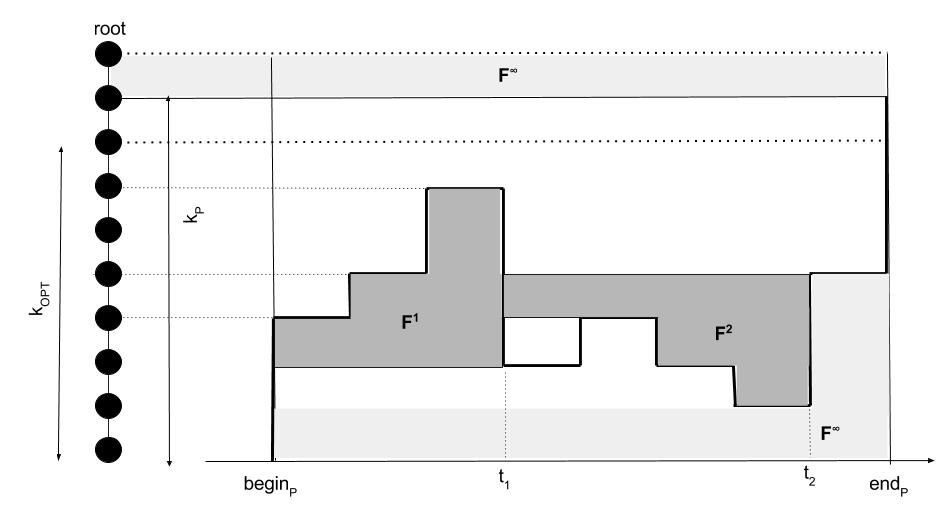
\includegraphics[width=\textwidth]{fields.jpg}
\end{center}
\end{figure}

\subsubsection{Shifting}
\paragraph{Up-shifting of negative requests}
\paragraph{Down-shifting of positive requests}

\subsubsection{Competitiveness of TRC}
\paragraph{Lower bound for OPT}
\paragraph{Main result}
\paragraph{Lower bound for competitive ratio}
